\section{Cache, Branch prediction and Translation Lookaside Buffer}

\subsection{Cache design and cache misses}

A cache is a small fast memory storage that holds the most recently used memory words.
Caches improves on the memory latency so memory access can be achieved within the demand of modern processors.
Modern memory systems usually have three caches: Level 1 (L1), Level 2 (L2) and Level 3 (L3). \citep[Section~4.5.1]{Tanenbaum}.

\begin{figure}
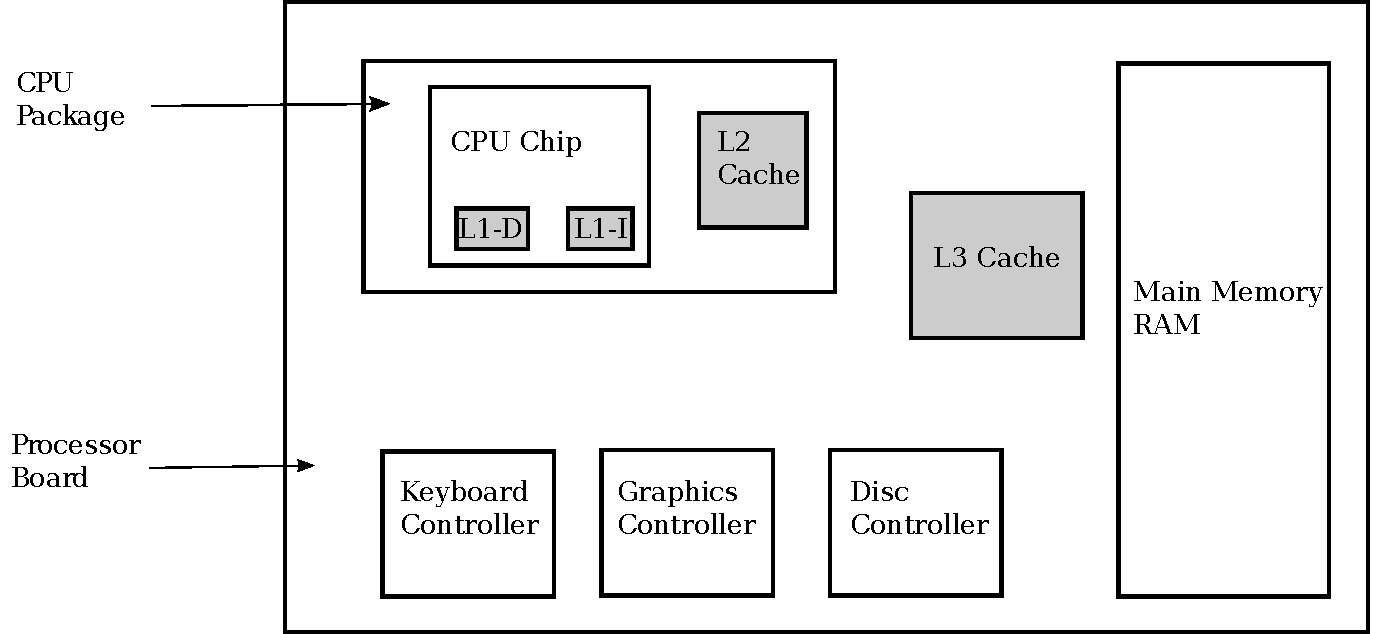
\includegraphics[width=\textwidth]{CacheLevels.pdf}
\caption{The three cache levels}
\label{fig:CacheLevels}
\end{figure}

Figure~\ref{fig:CacheLevels} shows how the three cache are placed in the relation to the CPU. 
The L1 cache resides on the CPU chip itself and usually has a size in the range from 16 KB to 128 KB and because it is placed directly on the CPU chip it is able to provide very fast memory access.
The L2 cache is placed next to the CPU chip on the CPU package and it is connected to the CPU via a high speed path. The L2 cache typically has a size between 512 KB and 1 MB which means that it can hold more data but is not able to provide as fast access as L1.
The L3 cache is placed on the processor board and usually has a size around 3 MB. Since it is placed further away from the cpu it is not able to provide as fast access as L1 and L2 but still much faster than fetching data from RAM.

All three caches are inclusive which means that L2 contains the data from L1 and L3 contains the data from L2.
This means that if data is evicted from L1 it will still reside in the L2 and L3 caches or if data is evicted from L2 it will still reside in L3. 
This is an advantage because it allows fast access to data even if it is evicted from L1 or L2. 
If the caches were not inclusive then it would result in a many more data requests to the main memory which is quite slow in relation to cache data access.

There are two types of address locality that the L1, L2 and L3 caches depends on; Spatial locality and Temporal locality.
Spatial locality occurs when memory locations that has addresses numerically similar to a recently accessed memory location are likely to be requested again very soon.
Temporal locality happens when memory locations that has been accessed recently are accessed again.
The cache exploits spatial locality by fetching more data than has been requested, assuming that it is possible to anticipate future requests.
Temporal locality is exploited by choosing what to evict on a cache miss and normally it is the data entries that has not been accessed recently that are evicted.

Data in the main memory is split into blocks of fixed size called \textit{cache-lines}. 
There are usually 4 to 64 consecutive bytes in a \textit{cache-line}. 
Some of these cache-lines are always present in the caches. 
If a requested word is in the cache a trip to main memory can be saved but if the word is not in the cache then a cache-line must be removed from the cache and the cache-line containing the word must be fetched from main memory or a lower level cache if one is present. 
This is called a \textbf{cache miss} and has a high penalty because fetching a new cache-line is expensive.
The general idea is to have the most heavily used cache-lines in the caches as often as possible to reduce the amount of cache misses.

\subsubsection{Cache associativity}
When designing a cache it is important to consider whether each cache-line can be stored in any cache slot or only in some of them.
There are three approaches to solving this problem; \textit{direct mapped cache}, \textit{n-way set-associative cache} and \textit{fully associative cache}. 

In a \textit{direct mapped cache} each cache-line can only be stored in a specific cache slot.
This means that two cache-lines cannot be mapped to the same slot simultaneously.
Given a memory address it is only necessary to look for it in one place in the cache and if it is not there then it is not in the cache. Using this approach consecutive memory lines are placed in consecutive cache slots. 
The problem with a \textit{direct mapped cache} is that since there are many more cache-lines in main memory than there are room for in the cache, many cache-lines ends up competing for the same slot. 
These competing cache-lines might end up constantly evicting each other which results in a substantial performance loss.

This problem can be fixed by using a \textit{n-way set-associative cache} which is a cache that allows \textit{n} entries for each cache-line.
This way if we have two cache-lines \textit{A} and \textit{B} and a slot is already occupied by \textit{A} while \textit{B} tries to use the same slot then \textit{A} does not have to be evicted because B has $n-1$ other slots to choose from.
If all \textit{n} slots are occupied then a cache-line from one of them has to be evicted.
The question then becomes: Which one?

A popular algorithm, that answers this question is called \textit{LRU (Least Recently Used)}.
It works by keeping a ordering of each set of slots that can be accessed from a given cache-line. 
When a cache-line that is present in the cache is accessed the LRU algorithm updates the list by marking the entry corresponding to the accessed cache-line into the most recently accessed one.
When an entry needs to be replaced it is the one at the end of the list that is evicted because it is the least recently used entry.

A \textit{fully associative cache} allows any cache-line to be saved in any cache slot but it is complicated and costly to implement in hardware because it for instance needs to keep an ordered LRU list which requires a lot of bookkeeping.

In the end the \textit{n-way set-associative cache} is the most popular choice because it has a good trade-off between implementation complexity and cache-hit rate.


\subsection{Branch Prediction and Misprediction}
Modern computers are highly pipelined and pipelining works best on linear code because then the fetch unit is able to read consecutive words from memory and also better make use of prefetching.

Programs are not linear though, but are full of branch instructions. There are unconditional branches and conditional branches. 
An example of a conditional branch is an \textit{if-statement} and an example of an unconditional branch is an \textit{else-statement} that is not followed by an if-statement as shown in figure~\ref{fig:branchexample} where \textit{BNE Else} is a conditional branch and \textit{BE Next} is an unconditional branch. 

\begin{figure}\begin{framed}
\begin{algorithmic}
\If{$i == 0$}
	\State $k = 1$
\Else
	\State $k = 2$
\EndIf
\end{algorithmic}
\vspace{0.3cm}
\noindent
A possible translation to assembly looks like this:
\vspace{0.3cm}
\begin{enumerate}
\item \itab{ } \tab{CMP $0,1$} \tab{: compare i to 0}
\item \itab{ } \tab{BNE Else} \tab{: branch to Else if not equal}
\item \itab{Then:} \tab{MOV $k,1$} \tab{: move 1 to k}
\item \itab{ } \tab{BR Next} \tab{: unconditional branch to Next}
\item \itab{Else:} \tab{MOV $k,2$} \tab{: move 2 to k}
\item \itab{Next:}
\end{enumerate}
\caption{Program fragment with conditional and unconditional branches}
\label{fig:branchexample}
\end{framed}
\end{figure}


Conditional branches poses a problem because the code splits in two possible directions and the fetcher needs to know which one to choose.
Unconditional branches does not split the code in two directions and therefore it should be clear what to fetch but that is not the case.
This is because fetching occurs before instruction decoding in the pipeline and as a consequence the fetcher has to decide what to fetch next before it knows what instruction it was just looking at.
When the fetcher knows, 1 cycle later, that the instruction was an unconditional branch it has already started fetching the next instruction.
Many pipelined machines therefore allow that next instruction to execute even though that is not the logical choice. This instruction is therefore usually used as a \textit{delay slot} meaning that it is an instruction with no effect like the NOP instruction.
The compiler can try to optimize this by replacing NOP with some useful instruction but it is usually not able to according to \citep[Section 4.5.2]{Tanenbaum}.



\subsection{Translation Lookaside Buffer misses}
